\section{Evaluation}

\label{sec:evaluation}
We conducted qualitative and quantitative studies  
to answer the following research questions:

\begin{enumerate}[label=\textbf{RQ\arabic*},leftmargin=*]
	\item How accurate is the labeling associations inference? 

	\item How safe is the labeling markup repair process?
	
	\item How scalable is the performance with the size of 
	real-world web forms? Is it suitable for real-time usage?
\end{enumerate}

In the following subsections, we discuss the details of the experiments that 
we designed to answer each research question, together with the results and discussions.

\subsection{RQ1: Inference Accuracy}\label{subsec:rq1}
In this question, the objective is to assess how accurate 
is the inference of the labeling associations in a given web form. 
We recall that, as per the ARIA standard, a web form is accessible 
if it has markup that correctly captures the labels on the form. 
Accordingly, the most important evaluation question is to 
assess how accurate are the inferred form labels. 

We evaluated this research question as follows. 
First, we collected 30 random subjects that were sourced 
from the Alexa top websites list~\cite{alexatop}. 
The way we selected the evaluation subjects are as follows. 
To start, we get a random subject url from the pool. 
We then load that url in a browser in order to inspect the website. 
This inspection process is conducted manually, and its goal is to 
find a page on the website that contains a web form. 
For each website, we manually inspect its various sections and pages 
until a web form is found. If no web forms are found within five minutes 
of manual examination, the subject is skipped and a new random url 
is obtained from the pool. The only additional criterion we have on web forms 
is that they are reachable without requiring registration or payment. 
This criterion was made in order to simplify the process of collecting 
subjects. The final list of subjects is shown in \Cref{table:subjects}, 
and the full urls are available online~\cite{tool-and-data}. 
The final list of subjects covers a variety of tasks from 
many categories of websites (e.g. news, education, commerce), 
with a varying number of elements in forms, ranging from 17 up to 1552, 
which covers around two orders of magnitude of form sizes. This 
variety of topics and size ranges helps in having a more 
representative and generalizable evaluation. 
Subsequently, we feed the web form to our approach and obtain 
the output labeling associations. We then examine each generated 
association and classify the results into true positives, 
false positives, and false negatives. 
In false positives, the inferred labeling association for 
a given field does not match the visually perceived labeling. 
For instance, in \Cref{fig:motivating-example}b, if the 
inferred labeling associates the selected radio button to 
the label `Yes`, then this is a false positive labeling, 
because it does not match the correct visually perceived 
labeling, which is the `No` option. 
Next, in true positives, the inferred labeling association 
for a given field correctly matches the visually perceived 
labeling. For instance, in \Cref{fig:motivating-example}b, 
if the inferred labeling associates the large text area 
input to the label `Message`, then this is a true positive labeling. 
Finally, false negatives are cases in which no labeling 
associations were inferred for a field that should have 
been associated with a label. For instance, in \Cref{fig:motivating-example}b,
if no labels were associated to the first text field input, 
then this is a false negative, because there should 
have been a label (i.e., `Name`). 

Finally, in order to have a more thorough and informative evaluation, we include a baseline in our experiments. 
While we could simply present the evaluation from just the approach 
itself, this would not provide context as to how it would 
perform compared to other potential solutions, and therefore 
adding a baseline helps in making the evaluation more meaningful. 
However, as discussed in the introduction, 
existing works only test the accessibility of markups, but do not 
conduct any inferences or repairs of form labeling~\cite{yesilada2019web, ukgov:audit:2018}. 
They assert that accessibility attributes are not empty, 
while the proposed analysis in this chapter infers what \emph{values}  
should be assigned to the form labeling attributes. 
Accordingly, no comparable tool exists that can be included in the evaluation, and 
therefore the next best option is to have a random selection process as the baseline. 
In this process, random elements from a given web form are selected. 
Next, a labeling association is generated to another randomly selected form element. 
This set of randomly selected elements and their associations 
is then taken to be the baseline.

%\noindent\begin{minipage}[t]{\linewidth}
\renewcommand{\arraystretch}{0.7}
\begin{table}
\caption{List of the 30 subjects used for evaluation.}
\label{table:subjects}
\centering
\begin{tabularx}{0.85\columnwidth}{llrr}
\hline
\small \textbf{Subject}  &  \small \textbf{Form} 						& \small \textbf{\# elements}  & \small \textbf{total \#} 		\\ %	& \textbf{total} \\ 
\small \textbf{}  &  \small \textbf{description} 			& \small \textbf{in form}  		& \small \textbf{elements} 			\\ %	& \textbf{size, KB} \\ 
\hline
\footnotesize wikipedia.org     & \footnotesize Page links search   					&	\footnotesize	45     						  &	\footnotesize 518				\\ %				&	227.1				      \\
\footnotesize opinionlab.com    & \footnotesize Experience feedback      &		\footnotesize 116     						  &	\footnotesize 136							\\ %	&	15.6				      \\     	   
\footnotesize zoom.us           & \footnotesize Live demo request      				&		\footnotesize 437     						  &	\footnotesize 924				\\ %				&	200.0		    \\           
\footnotesize netflix.com       & \footnotesize New titles suggestion      			&	   \footnotesize 17     						  &	\footnotesize 432			\\ %			&	148.6			 \\            
\footnotesize microsoft.com     & \footnotesize Careers support ticket      		&		\footnotesize 86     						  &	\footnotesize 444				\\ %		&	140.6			      \\           
\footnotesize dropbox.com       & \footnotesize Business account inquiry      		&		\footnotesize 398     						  &	\footnotesize 721			\\ %			&	130.2		      \\           
\footnotesize stackoverflow.com & \footnotesize Help center      						&     \footnotesize 106     						  &	\footnotesize 743				\\ %			&	106.7		      \\            
\footnotesize etsy.com          & \footnotesize Product design careers      		&		\footnotesize 68     						  &	\footnotesize 340				\\ %			&	347.9		      \\            
\footnotesize zendesk.com       & \footnotesize Customer service inquiry      		&	   \footnotesize 428     						  &	\footnotesize 1323			\\ %			&	209.6		      \\            
\footnotesize bing.com          & \footnotesize  Search customization     &	   \footnotesize 1552     					  &	\footnotesize 1642						\\ %		&	289.0		      \\          
\footnotesize github.com        & \footnotesize Account support request     		&	   \footnotesize 229     						  &	\footnotesize 283				\\ %			&	42.8	      \\           
\footnotesize intuit.com        & \footnotesize Career events sign-up      			&	   \footnotesize 326     						  &	\footnotesize 1293			\\ %		&	201.5		      \\           
\footnotesize salesforce.com    & \footnotesize Website quality feedback      		&	   \footnotesize 102     						  &	\footnotesize 764			\\ %		&	279.9				      \\            
\footnotesize indeed.com        & \footnotesize Account registration      			&	   \footnotesize 54     						  &	\footnotesize 222				\\ %		&	47.0				      \\            
\footnotesize paypal.com        & \footnotesize Search for jobs      					&		\footnotesize 144     						  &	\footnotesize 410			\\ %		&	48.55				      \\            

\footnotesize coursera.org		& \footnotesize Services inquiry	&  \footnotesize 569  & \footnotesize 1210 \\
\footnotesize glassdoor.com		& \footnotesize Sales specialist contact	& \footnotesize 1536	& \footnotesize 1864	\\
\footnotesize insiderintelligence.com	& \footnotesize Subscription request &	\footnotesize 391	& \footnotesize 1019	\\
\footnotesize formstack.com		& \footnotesize Violations reporting	& \footnotesize 126	& \footnotesize 182	\\
\footnotesize dailymail.co.uk	& \footnotesize Message board help	& \footnotesize 45	& \footnotesize 986	\\

\footnotesize squarespace.com	& \footnotesize Press contact	& \footnotesize 33	& \footnotesize 725	\\
\footnotesize elsevier.com		& \footnotesize Advertising request	& \footnotesize 437	& \footnotesize 940	\\
\footnotesize hootsuite.com		& \footnotesize Community enrolment	& \footnotesize 61	& \footnotesize 560	\\
\footnotesize flickr.com		& \footnotesize Support ticket request	& \footnotesize 243	& \footnotesize 348	\\
\footnotesize goodreads.com		& \footnotesize Advertising inquiry	& \footnotesize 75	& \footnotesize 551	\\

\footnotesize slack.com			& \footnotesize Sales contact	& \footnotesize 461	& \footnotesize 1087	\\
\footnotesize evernote.com		& \footnotesize Teams products inquiry	& \footnotesize 298	& \footnotesize 730	\\
\footnotesize udemy.com			& \footnotesize Demo request	& \footnotesize 50	& \footnotesize 241	\\
\footnotesize blackboard.com	& \footnotesize Personalized experience	& \footnotesize 641	& \footnotesize 838	\\
\footnotesize mailchimp.com		& \footnotesize Report compliance issues	& \footnotesize 58	& \footnotesize 1209	\\  

\end{tabularx}
\end{table}
%\end{minipage}

\subsubsection{Results and Discussion}
\Cref{table:rq1} shows the results of evaluating the accuracy 
of inferring web form labeling. 
The table has two groups of columns, ``Proposed approach'' 
and ``Baseline'', 
showing the accuracy of inference for both methods, respectively. 
The key outcome of this table is the F-1 measure, 
which is at 89\% for the proposed approach. 
This indicates a rather effective inference process. 
Precision and recall were comparable, at 88\% and 89\%, 
respectively. 
\Cref{fig:label-pairs} shows a sample of the inferred labeling 
associations corresponding to the motivating example. Each 
entry represents a mapping from a particular field to a particular label.

%\noindent\begin{minipage}[t]{\linewidth}
\renewcommand{\arraystretch}{0.7}
\begin{table}[t]
\caption{Evaluation of the inference accuracy of labeling associations.}
\label{table:rq1}
\centering
\begin{tabularx}{0.85\columnwidth}{p{0.2\textwidth}rrr|rrr}
\hline
                  & \multicolumn{3}{c|}{\textbf{\small Proposed}}                                      & \multicolumn{3}{c}{\textbf{\small Baseline}}                                          \\
                  & \multicolumn{3}{c|}{\textbf{\small approach}}                                      & \multicolumn{3}{c}{}                                                \\
\hline
\textbf{\small Subject}           & \multicolumn{1}{c}{\textbf{\small TP}} & \multicolumn{1}{c}{\textbf{\small FP}} & \multicolumn{1}{c|}{\textbf{\small FN}} & \multicolumn{1}{c}{\textbf{\small TP}} & \multicolumn{1}{c}{\textbf{\small FP}} & \multicolumn{1}{c}{\textbf{\small FN}}  \\ 
\hline
\small wikipedia.org     & 3                       & 0                       & 0                       & 0                       & 5                       & 1                        \\
\small opinionlab.com    & 6                       & 2                       & 0                       & 0                       & 11                      & 1                        \\
\small zoom.us           & 12                      & 0                       & 2                       & 0                       & 13                      & 4                        \\
\small netflix.com       & 3                       & 0                       & 2                       & 1                       & 4                       & 3                        \\
\small microsoft.com     & 5                       & 0                       & 0                       & 0                       & 15                      & 0                        \\
\small dropbox.com       & 9                       & 0                       & 1                       & 0                       & 7                       & 4                        \\
\small stackoverflow.com & 4                       & 1                       & 0                       & 0                       & 6                       & 1                        \\
\small etsy.com          & 3                       & 0                       & 2                       & 0                       & 2                       & 3                        \\
\small zendesk.com       & 6                       & 0                       & 0                       & 0                       & 9                       & 1                        \\
\small bing.com          & 11                      & 7                       & 1                       & 0                       & 5                       & 4                        \\
\small github.com        & 5                       & 0                       & 0                       & 0                       & 9                       & 2                        \\
\small intuit.com        & 6                       & 0                       & 0                       & 1                       & 7                       & 2                        \\
\small salesforce.com    & 3                       & 1                       & 1                       & 0                       & 8                       & 1                        \\
\small indeed.com        & 5                       & 2                       & 1                       & 0                       & 6                       & 2                        \\
\small paypal.com        & 4                       & 0                       & 0                       & 1                       & 3                       & 1                        \\
\small coursera.org			& 12	& 0		& 1		& 0		& 6		& 5 \\
\small glassdoor.com			& 7		& 0		& 3		& 0		& 5		& 3 \\
\small insiderintelligence.com	& 7		& 3		& 0		& 0		& 4		& 6 \\
\small formstack.com			& 6		& 1		& 0		& 0		& 3		& 5 \\
\small dailymail.co.uk			& 8		& 0		& 1		& 1		& 4		& 3 \\
\small squarespace.com			& 5		& 1		& 0		& 1		& 5		& 1 \\
\small elsevier.com			& 15	& 1		& 2		& 0		& 6		& 10 \\
\small hootsuite.com			& 5		& 0		& 0		& 0		& 4		& 1 \\
\small flickr.com				& 6		& 1		& 2		& 0		& 3		& 6 \\
\small goodreads.com			& 7		& 0		& 1		& 0		& 2		& 5 \\
\small slack.com				& 10	& 2		& 2		& 0		& 8		& 4 \\
\small evernote.com			& 6		& 1		& 0		& 0		& 4		& 3 \\
\small udemy.com				& 7		& 0		& 0		& 1		& 3		& 3 \\
\small blackboard.com			& 13	& 3		& 1		& 0		& 5		& 11 \\
\small mailchimp.com			& 8		& 1		& 1		& 0		& 6		& 4 \\
\hline
						& Prec.						  & Rec.							 & F1							   & Prec.						  & Rec.							 & F1				 \\
						& 88.4\%						  & 89.6\%						 & 89.0\%						& 3.3\%					 	  & 5.7\%						 & 4.1\%			 \\

\end{tabularx}
\end{table}
%\end{minipage}
























In order to further understand the limitations of the approach, 
we investigated the false positive and false negative cases. 
We identified a few trends. First, false positives occurred in 
forms that had visual prominence cues that did not follow the 
proposed optimization model (\Cref{{subsec:obj}}). In these 
cases, the forms had a high ratio of texts relative to fields 
and all the texts had similar visual prominence cues. This 
resulted in the optimization process yielding suboptimal 
labeling associations. False positives also occurred in cases 
where, in addition to the aforementioned similarity in visual 
prominence, the visual layout was dense, which made it difficult 
to compensate for the layout density using visual prominence information. 

As for the false negatives, the most predominant case was due to 
non-standard form elements. That is, these cases did not follow 
the normal practice of using input tags to indicate form fields. 
The most common example of this case is Captcha elements 
(e.g.,~``I'm a human" checkboxes), which are designed on purpose to avoid 
being detected by automated tools as form fields.  
Such elements are only styled to appear, for instance, as a 
checkbox when observed by sighted users. For these reasons, 
existing studies~\cite{moreno2014captcha,noorjahan2019bio} have 
also confirmed these hindrances of accessibility due to Captcha elements. 
The proposed approach is incapable of handling these cases. 
For future work, a potential solution to this problem might include 
formulating another set of visual cues to detect the missed cases, 
or exploring the use of a deep learning detector.   

We also examined the effect of form size on the inference accuracy, 
as shown in \Cref{fig:stratified}. The figure shows the average F1 
score of inference for three different groups of form sizes, which 
are the 0 to 33, 33 to 66, and 66 to 100 percentile of form sizes as 
measured by the number of DOM elements in the form. First, we note 
that the first group had slightly lower inference accuracy compared 
to the second group. But we do know that the number of false positives have stayed the same, and therefore the lower accuracy can be attributed to the arithmetic of computing accuracy, where a single inference error in a form with a small number of elements would impact the accuracy more so than a single inference error among a large number of form elements. Second, we note that the lowest accuracy was for the last group (i.e., largest forms). This is due 
to the observation mentioned in the preceding paragraphs, where the 
larger forms tend to have a more dense visual layout, which reduced the 
quality of the optimization decisions as the cues became less 
discriminating due to the higher layout density. However, 
the observed reduction in accuracy is not that significant, and we 
emphasize that all the aforementioned observations are relative in 
nature with respect to the other size groups. Accordingly, the key 
observation of this evaluation is that the inference accuracy remains 
relatively stable across size ranges in \Cref{fig:stratified}.

\begin{figure}
    \noindent
	\begin{minipage}[c]{.97\columnwidth}
        \centering
        \begin{lstlisting}[language={JavaScript},frame=ltbr,aboveskip=1.1em,basicstyle={\linespread{0.8}\footnotesize\ttfamily},]		
{	// associations.json
	// each entry is xpaths of field -> label 

	".../form/textarea[@id='bx_3978']": 
			".../form/div[1]/p", // <p>Message</p>
	
	".../form/input[@id='vr_9481']": 
			".../form/section[1]/div[1]/p", // <p>Name</p>
	
	".../form/select[@id='frq']": 
			".../form/section[2]/div[2]/p", // <p>How often ...</p>
	
	// remaining elements ...
}\end{lstlisting}
    \end{minipage} \hfill
\caption{Sample of the generated association decisions output (corresponds to \Cref{fig:motivating-example}).}
    \label{fig:label-pairs}
\end{figure}

\subsection{RQ2: Markup Safety}\label{subsec:rq2}
In the previous research question, we examined how accurate the labeling 
association inference is. 
Once that aspect has been evaluated, we need to examine whether 
the insertion or augmentation of the inferred associations into the 
DOM is safe. 
The rationale for evaluating this aspect is that we want to make 
sure that any markup repairs applied to a page does not 
cause any unintended or unaccounted for breakages or failures to the page. 

We evaluated this research question as follows. 
First, we continued using the same test subjects used in the first 
research question. Each subject is then loaded in a browser 
and had their labeling associations inferred and the DOM repaired. 
To assess the safety, we check two different aspects. First, 
a visual check is made comparing images of the page before and 
after the repair. The rationale is to assess whether the generated 
markup would cause unintended breakage to the rendering of the page. 
Second, a functionality check is made. Here, we randomly manipulate 
the form (e.g., we select various radio options, expand different drop down menus) to assess whether the generated markup caused  unintended breakage to the form. Breakages might occur, for instance, if the generated markups are incorrect, or break some element or attribute dependencies in the script of the page. Finally, we note down the outcome (i.e., pass or fail), and note down the number of failures. 


\subsubsection{Results and Discussion}
\Cref{table:rq2} shows the results of evaluating the safety of 
the markup repair. For each subject, the columns show the 
outcome of the safety check and the number of failures. Subjects 
for which no failures were observed have `-' under the number of 
failures column. For most subjects, we did not observe any failures. 
For two of the subjects, as shown in \Cref{table:rq2}, we did 
observe failures. In both these cases, the DOM repair process  failed. The reason for these failures is locator breakages. This occurs 
because after the labeling association for a field is determined, 
locators are used locate the field in the DOM, then insert the markup 
repairs at that location. But in the case of the observed failures, 
the locators became stale, where locators that were 
previously valid become unusable. This occurred because the subject's 
DOM was highly dynamic and therefore the DOM has changed 
since the time the locator was acquired. In this work we used DOM 
locators in the form xpath strings. The issue of stale locators 
and possible approaches to address them have been also reported in 
other web testing and analysis works~\cite{leotta2016robula, kirinuki2019color} 
and is still an open research problem. 
For future work, we plan to explore different possibilities to capture 
the locators and address these issues. One option would be devising a 
more robust timing strategy at which to capture the locators in order to 
minimize the probability of going stale. Another option would be using 
visual locators instead of DOM locators. 
 
%\noindent\begin{minipage}[t]{\linewidth}
\begin{table}[t]
\caption{Evaluation of accessibility markup augmentation safety.}
\label{table:rq2}
\centering
\begin{tabular}{llr}
\hline
\textbf{Subject}    & \textbf{Outcome} 		&\textbf{\# failures} \\ 
\hline
paypal.com        	& fail      			&		3             \\
intuit.com        	& fail      			&		2             \\
remaining subjects	& pass	  				& 		- 			  \\
\hline
\end{tabular}
\end{table}
%\end{minipage}    

\subsection{RQ3: Runtime Scalability}\label{subsec:rq3}
After evaluating the accuracy and safety aspects in the previous 
research question, this question examines the runtime performance (i.e., 
total time of execution). 
The rationale for evaluating this question is as follows. 
First, since a couple of aspects in the optimization formulation 
are combinatorial in nature, we wanted to assess whether or not this 
is going to cause any performance penalty, and more importantly how does 
the performance scale with the size of forms. 
Second, since the goal of this work is to make web forms accessible, 
it would be useful to know if the runtime performance is good enough 
if this approach were to be used for real-time repair by end users 
during their browsing activities. 

We evaluated this research question as follows. 
For each subject, we record the number of DOM elements in the forms 
as a measure of form size. We are measuring the elements in the form 
since our approach only focuses on form regions within the page, 
and is therefore not impacted by the rest of the page.
This will be used to measure how does the runtime scale with form size. 
Then, the total runtime is measured from the moment the subject is loaded 
until the final DOM markup is augmented. 

\subsubsection{Results and Discussion}
\Cref{fig:rq3} shows the results of the runtime performance evaluation. 
The x-axis is semi-log and shows the number of DOM elements within 
the form. The y-axis is linear and shows the runtime in milliseconds. 

The average runtime is $1667 \pm 532$ milliseconds. Minimum and 
maximum runtimes are 1044 and 2733 milliseconds, respectively. 
The data range of DOM elements covers around two orders of magnitude 
of form sizes, making it suitable for assessing scalability.
The runtime scales roughly linearly with the size of the DOM, 
indicating good scalability with respect to form complexity.  
We recall that we are implementing the optimization in the Lpsolve~\cite{lpsolve} 
solver. While the solver is a good fit for the type of optimization 
we are conducting, it is known to be lacking in terms of runtime 
performance~\cite{luppold2018evaluating}. Accordingly, while the 
observed average performance of around 1.6 seconds is arguably 
suitable for run-time repair, the performance will likely improve 
further when more capable solvers are used, and therefore the 
current evaluation is a conservative estimate. The key outcome, 
however, remains the same, which is that the proposed web form 
analysis scales linearly with respect to form complexity. This 
provides some indication that the formulated optimization problem 
and constraints do not practically result in a combinatorial 
explosion that would cause computationally prohibitive analysis.   

\begin{figure}
	\centering
	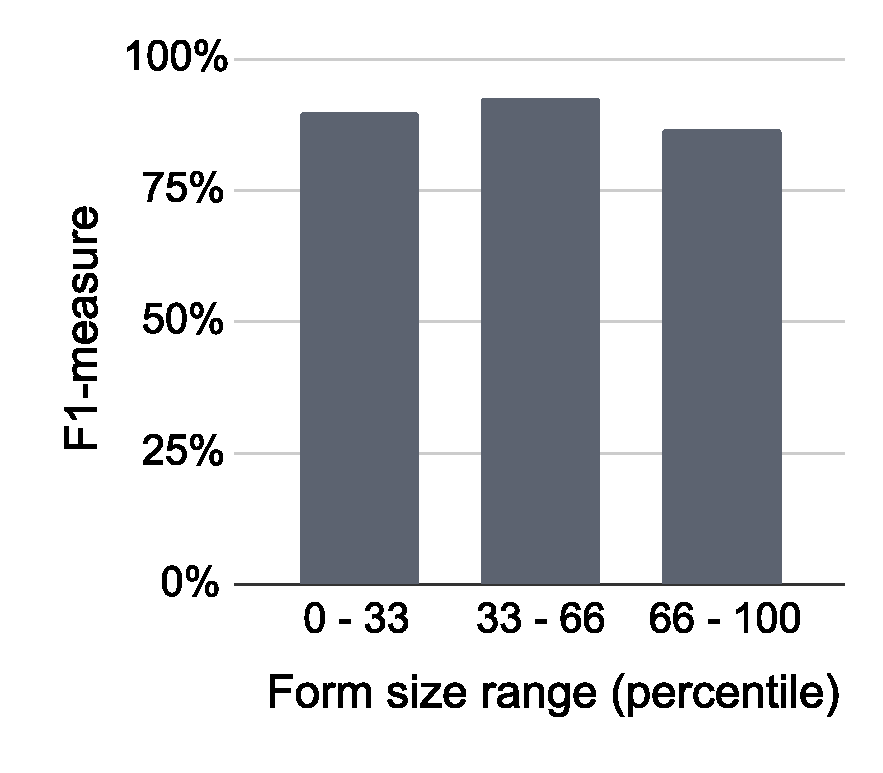
\includegraphics[width=0.45\linewidth,trim=11mm 9mm 7mm 7mm,clip]{accessibility_repair/figures/stratified.pdf}
	\caption{Comparison of labeling inference F1-measure for different form size ranges.}
	\label{fig:stratified}
\end{figure}

\subsubsection{Threats to validity}
In order to avoid any selection bias, 
we chose test subjects (i.e., web sites) 
randomly with the mentioned 
criteria in \Cref{subsec:rq1}. 
The subjects cover diverse categories 
(e.g. news, education, commerce), 
with around two orders of magnitude of 
form sizes, ranging from 17 up to 1552 elements.
This diversity of topics and sizes helps in 
ensuring subjects are representative 
of real-world scenarios, thereby mitigating the 
external validity of the study by making the 
results generalizable.
To make the study replicable and mitigate researcher bias, 
we made available online a link to our tool 
implementation and evaluation data~\cite{tool-and-data}.



